% =====================================================================
\chapter{Régression et estimation}
\label{ch:2}
% =====================================================================

\section{Objectifs et organisation du chapitre}

\paragraph{Objectifs.} Le chapitre~1 a montré que le ratio de couverture à variance minimale est une pente de régression. Ce chapitre donne les outils pour estimer ces pentes correctement et pour savoir quand faire confiance au résultat. À la fin du chapitre, vous saurez : (1) dériver les moindres carrés ordinaires sous forme scalaire et matricielle ; (2) énoncer les hypothèses qui rendent l'estimateur sans biais et ses erreurs-types valides ; (3) corriger les erreurs-types quand les résidus sont autocorrélés (Newey-West) ; (4) expliquer pourquoi régresser $Y$ sur $X$ ne donne pas le même ratio que régresser $X$ sur $Y$, et calculer la régression orthogonale ; (5) écrire et maximiser une vraisemblance, en particulier celle de l'AR(1) ; (6) corriger le biais de petit échantillon du coefficient autorégressif.

\paragraph{Code.} Toutes les vérifications sont dans \texttt{code/ch02/ch02\_regression.py} (expériences E1 à E5), résultats dans \texttt{code/ch02/results.json}.

% =====================================================================
\section{Le modèle linéaire et les moindres carrés}
% =====================================================================

\subsection{Cas d'une seule variable explicative}

On observe $n$ couples $(x_i, y_i)$ et l'on postule $y_i = a + b\,x_i + e_i$, où $e_i$ est un résidu. Les moindres carrés ordinaires (MCO) choisissent $(a,b)$ qui minimisent la somme des carrés des résidus
\[
S(a,b) = \sum_{i=1}^n (y_i - a - b x_i)^2.
\]

\begin{proposition}\label{c2:prop:ols1}
Le minimum est atteint en $\hat b = \dfrac{\sum_i (x_i-\bar x)(y_i-\bar y)}{\sum_i (x_i-\bar x)^2}$ et $\hat a = \bar y - \hat b\,\bar x$.
\end{proposition}
\begin{proof}
$S$ est une fonction convexe de $(a,b)$ (somme de carrés de fonctions affines), donc son minimum annule ses deux dérivées partielles.
\begin{align*}
\frac{\partial S}{\partial a} &= -2\sum_i (y_i - a - b x_i) = 0 \;\Rightarrow\; \sum_i y_i = n a + b\sum_i x_i \;\Rightarrow\; a = \bar y - b\bar x.\\
\frac{\partial S}{\partial b} &= -2\sum_i x_i(y_i - a - b x_i) = 0.
\end{align*}
On remplace $a$ par $\bar y - b\bar x$ dans la seconde équation : $\sum_i x_i\big((y_i-\bar y) - b(x_i-\bar x)\big) = 0$. Comme $\sum_i \bar x\,(y_i - \bar y) = 0$ et $\sum_i\bar x\,(x_i-\bar x) = 0$, on peut remplacer $x_i$ par $x_i - \bar x$ devant la parenthèse sans changer la somme : $\sum_i (x_i-\bar x)(y_i-\bar y) = b\sum_i(x_i-\bar x)^2$, d'où $\hat b$.
\end{proof}

En divisant numérateur et dénominateur par $n-1$, on reconnaît $\hat b = \widehat{\Cov}(X,Y)/\widehat{\Var}(X)$ : c'est la version empirique du ratio de couverture optimal de la proposition~\ref{c1:prop:hedge}.

\subsection{Forme matricielle}

Avec $k$ variables explicatives (dont la constante), on empile les observations : $y \in \R^n$, $X \in \R^{n\times k}$ (une ligne par date, une colonne par variable, la première colonne remplie de 1), $\beta \in \R^k$. Le modèle s'écrit $y = X\beta + \varepsilon$.

\begin{proposition}[Équations normales]\label{c2:prop:olsmat}
Si $X^\top X$ est inversible, l'estimateur des MCO est $\hat\beta = (X^\top X)^{-1}X^\top y$, et les résidus $e = y - X\hat\beta$ vérifient $X^\top e = 0$.
\end{proposition}
\begin{proof}
La somme des carrés vaut $S(b) = (y-Xb)^\top(y-Xb) = y^\top y - 2b^\top X^\top y + b^\top X^\top X b$ (on a utilisé $y^\top Xb = b^\top X^\top y$, car c'est un nombre, égal à son transposé). Le gradient par rapport à $b$ est $\nabla S = -2X^\top y + 2X^\top X b$ (règles $\nabla_b(b^\top c) = c$ et $\nabla_b(b^\top Ab) = 2Ab$ pour $A$ symétrique). L'annuler donne $X^\top X\hat\beta = X^\top y$, puis $\hat\beta = (X^\top X)^{-1}X^\top y$. Enfin $X^\top e = X^\top y - X^\top X\hat\beta = 0$ par les équations normales elles-mêmes.
\end{proof}

\begin{intuition}
$X\hat\beta$ est l'ombre de $y$ projetée sur le plan engendré par les colonnes de $X$, comme l'ombre d'un bâton au soleil de midi sur le sol. Le résidu $e$ est la partie verticale, perpendiculaire au sol : c'est exactement ce que dit $X^\top e = 0$. En \emph{pairs trading}, le résidu de la régression de $Y$ sur $X$ est le \emph{spread} : la partie de $Y$ que $X$ n'explique pas.
\end{intuition}

\paragraph{Qualité d'ajustement.} Le coefficient de détermination $R^2 = 1 - \sum e_i^2/\sum(y_i-\bar y)^2$ mesure la part de la variance de $y$ expliquée. Avec une seule variable explicative, $R^2 = \hat\rho_{XY}^2$.

\begin{codebox}[ — E1, données réelles KO et PEP]
\textbf{Hypothèse :} les formules écrites à la main donnent les mêmes résultats que \texttt{statsmodels}. \textbf{Protocole :} régression du cours de clôture de Coca-Cola sur celui de PepsiCo, 500 séances (octobre 2024 à octobre 2026). \textbf{Résultats :} $\hat a = 105{,}23$ (erreur-type $4{,}68$), $\hat b = -0{,}2176$ (erreur-type $0{,}0319$), $R^2 = 0{,}0855$, identiques à \texttt{statsmodels} à $4\times10^{-12}$ près ; la plus grande composante de $X^\top e$ vaut $10^{-7}$ (zéro numérique). \textbf{Lecture :} sur ces deux années, les cours de KO et PEP ont évolué en sens opposés (KO a monté, PEP a baissé) ; la \og paire classique\fg{} des manuels n'avait aucune relation positive en niveau. Nous y reviendrons aux chapitres~4 et~7.
\end{codebox}

% =====================================================================
\section{Propriétés statistiques de l'estimateur}
% =====================================================================

\subsection{Hypothèses et absence de biais}

Les propriétés de $\hat\beta$ reposent sur des hypothèses sur le terme d'erreur $\varepsilon$ :
\begin{enumerate}[label=(H\arabic*)]
\item \emph{linéarité} : $y = X\beta + \varepsilon$ ;
\item \emph{rang plein} : $X^\top X$ inversible (aucune variable n'est combinaison linéaire des autres) ;
\item \emph{exogénéité} : $\E[\varepsilon \mid X] = 0$ ;
\item \emph{homoscédasticité et absence d'autocorrélation} : $\E[\varepsilon\varepsilon^\top \mid X] = \sigma^2 I_n$.
\end{enumerate}

\begin{proposition}\label{c2:prop:unbiased}
Sous (H1)–(H3), $\E[\hat\beta\mid X] = \beta$. Sous (H1)–(H4), $\Var(\hat\beta\mid X) = \sigma^2(X^\top X)^{-1}$.
\end{proposition}
\begin{proof}
On remplace $y$ par $X\beta+\varepsilon$ : $\hat\beta = (X^\top X)^{-1}X^\top(X\beta+\varepsilon) = \beta + (X^\top X)^{-1}X^\top\varepsilon$. En prenant l'espérance conditionnelle à $X$ et en utilisant (H3) : $\E[\hat\beta\mid X] = \beta + (X^\top X)^{-1}X^\top\E[\varepsilon\mid X] = \beta$. Pour la variance, $\hat\beta - \beta = A\varepsilon$ avec $A = (X^\top X)^{-1}X^\top$, donc $\Var(\hat\beta\mid X) = A\,\E[\varepsilon\varepsilon^\top\mid X]\,A^\top = \sigma^2AA^\top = \sigma^2(X^\top X)^{-1}X^\top X(X^\top X)^{-1} = \sigma^2(X^\top X)^{-1}$.
\end{proof}

On estime $\sigma^2$ par $\hat\sigma^2 = e^\top e/(n-k)$ ; la division par $n-k$ plutôt que $n$ corrige le fait que $k$ paramètres ont été ajustés sur les mêmes données. Le théorème de Gauss-Markov ajoute que, sous (H1)–(H4), $\hat\beta$ a la plus petite variance parmi tous les estimateurs linéaires sans biais.

\subsection{Le test de Student et ses conditions}

La statistique $t_j = \hat\beta_j/\widehat{\mathrm{se}}(\hat\beta_j)$, où $\widehat{\mathrm{se}}$ est la racine du $j$-ème terme diagonal de $\hat\sigma^2(X^\top X)^{-1}$, suit approximativement une loi normale centrée réduite si $\beta_j = 0$. Ce résultat exige (H4). Or les séries financières violent souvent (H4) : un \emph{spread} qui revient lentement à la moyenne a des résidus fortement autocorrélés. Le chapitre~1 a montré le cas extrême (régression fallacieuse, section~\ref{c1:sec:spurious}) ; même avec des séries stationnaires, l'autocorrélation fausse les erreurs-types.

\subsection{Erreurs-types robustes : Newey-West}

Sans (H4), la variance exacte de $\hat\beta$ est
\[
\Var(\hat\beta\mid X) = (X^\top X)^{-1}\Big(\sum_{t}\sum_{s} x_t x_s^\top\,\E[\varepsilon_t\varepsilon_s]\Big)(X^\top X)^{-1},
\]
où $x_t$ est la $t$-ème ligne de $X$ écrite en colonne. La partie centrale, appelée \og viande\fg{} du \og sandwich\fg, contient les covariances croisées des erreurs. \citet{neweywest1987} l'estiment par
\[
\hat\Omega = \hat\Gamma_0 + \sum_{j=1}^{L}\Big(1-\frac{j}{L+1}\Big)\big(\hat\Gamma_j + \hat\Gamma_j^\top\big), \qquad \hat\Gamma_j = \sum_{t=j+1}^{n} e_t e_{t-j}\,x_t x_{t-j}^\top,
\]
avec $L$ retards. Les poids $1 - j/(L+1)$ décroissent linéairement et garantissent que la matrice estimée reste positive.

\begin{codebox}[ — E5, erreurs-types naïves contre Newey-West]
\textbf{Hypothèse :} quand $x$ et les résidus sont tous deux autocorrélés, le test de Student naïf rejette à tort \og pente nulle\fg{} beaucoup plus souvent que 5\,\%, et Newey-West corrige en partie. \textbf{Protocole :} 2\,000 répétitions ; $x$ et $u$ indépendants, chacun AR(1) avec $\varphi = 0{,}9$ ; $y = 1 + 0\cdot x + u$ ; $n = 250$. \textbf{Résultats :} taux de rejet à 5\,\% : $51{,}6\,\%$ en naïf, $27{,}1\,\%$ avec Newey-West à 4 retards (règle usuelle $L = \lfloor 4(n/100)^{2/9}\rfloor$), $17{,}9\,\%$ avec 20 retards.
\end{codebox}

\begin{pitfall}
Le test naïf trouve une relation significative une fois sur deux entre deux séries indépendantes. Newey-West améliore nettement les choses mais reste loin des 5\,\% nominaux quand la persistance est forte et l'échantillon court. Règle pratique : ne jamais sélectionner une paire ou un signal sur la base d'un $t$ de Student calculé sur des séries persistantes ; utiliser les tests dédiés (chapitres~3 et~4), des erreurs-types robustes et, surtout, une validation hors échantillon (chapitre~16).
\end{pitfall}

% =====================================================================
\section{Quelle variable expliquer ? L'asymétrie de la régression}
% =====================================================================

\subsection{Deux régressions, deux ratios}

Pour un \emph{pairs trade}, il faut choisir quelle jambe joue le rôle de $Y$. Ce choix n'est pas neutre.

\begin{proposition}\label{c2:prop:asym}
Soit $\hat\beta_{Y|X}$ la pente de $Y$ sur $X$ et $\hat\beta_{X|Y}$ celle de $X$ sur $Y$. Alors $\hat\beta_{Y|X}\,\hat\beta_{X|Y} = \hat\rho_{XY}^2$, donc $1/\hat\beta_{X|Y} = \hat\beta_{Y|X}/\hat\rho_{XY}^2$.
\end{proposition}
\begin{proof}
D'après la proposition~\ref{c2:prop:ols1}, $\hat\beta_{Y|X} = \hat s_{XY}/\hat s_X^2$ et, par symétrie, $\hat\beta_{X|Y} = \hat s_{XY}/\hat s_Y^2$. Leur produit vaut $\hat s_{XY}^2/(\hat s_X^2\hat s_Y^2) = \hat\rho_{XY}^2$.
\end{proof}

Si l'on régresse $X$ sur $Y$ puis qu'on inverse la pente pour obtenir un ratio \og en unités de $X$ par unité de $Y$\fg, on obtient un ratio plus grand d'un facteur $1/\hat\rho^2$. Avec $\rho = 0{,}6$, l'écart est de 178\,\%. Seule une corrélation parfaite rend les deux choix équivalents.

\begin{intuition}
Les MCO ne mesurent les erreurs que dans une direction : verticalement quand on explique $Y$, horizontalement quand on explique $X$. Le bruit de la variable placée à droite (la variable explicative) \og aplatit\fg{} la pente vers zéro. C'est l'effet dit d'\emph{atténuation}.
\end{intuition}

\subsection{La régression orthogonale}

Pour traiter les deux actifs symétriquement, on minimise la somme des distances \emph{perpendiculaires} à la droite, ce qui revient à minimiser
\[
g(b) = \frac{s_{YY} - 2b\,s_{XY} + b^2 s_{XX}}{1+b^2},
\]
où $s_{XX}$, $s_{YY}$, $s_{XY}$ sont les variances et la covariance empiriques. En effet, la distance perpendiculaire d'un point à la droite $y = a + bx$ est $|y - a - bx|/\sqrt{1+b^2}$.

\begin{proposition}[Pente orthogonale]\label{c2:prop:tls}
Si $s_{XY} > 0$, le minimum de $g$ est atteint en
\[
\hat b_{\perp} = \frac{(s_{YY}-s_{XX}) + \sqrt{(s_{YY}-s_{XX})^2 + 4s_{XY}^2}}{2\,s_{XY}}.
\]
\end{proposition}
\begin{proof}
Écrivons $g = N/D$. La dérivée s'annule quand $N'D = ND'$, soit
$(-2s_{XY} + 2bs_{XX})(1+b^2) = 2b\,(s_{YY} - 2bs_{XY} + b^2s_{XX})$.
En développant les deux membres, les termes en $b^3s_{XX}$ s'annulent et il reste
$-2s_{XY} + 2s_{XY}b^2 + 2b(s_{XX} - s_{YY}) = 0$, soit l'équation du second degré $s_{XY}b^2 + (s_{XX}-s_{YY})b - s_{XY} = 0$. Son discriminant $(s_{XX}-s_{YY})^2 + 4s_{XY}^2$ est positif ; des deux racines, celle avec le signe $+$ est de même signe que $s_{XY}$ et correspond au minimum (l'autre est le maximum, la direction perpendiculaire).
\end{proof}

La pente orthogonale est la direction du premier vecteur propre de la matrice de covariance de $(X,Y)$ : c'est déjà une analyse en composantes principales, que l'on retrouvera au chapitre~10. Son défaut : elle dépend des unités (doubler le prix de $X$ change le résultat), d'où l'usage fréquent de log-prix ou de prix normalisés.

\begin{codebox}[ — E2, asymétrie et régression orthogonale]
\textbf{Simulation} (vrai $\beta = 1{,}5$, $X$ marche aléatoire, écart AR(1) de paramètre $0{,}9$, $n = 500$, 1\,000 répétitions) : MCO de $Y$ sur $X$ : moyenne $1{,}4986$ (écart-type $0{,}059$) ; inverse de la pente de $X$ sur $Y$ : $1{,}5642$ ($0{,}074$) ; régression orthogonale : $1{,}5445$ ($0{,}067$). \textbf{Variables stationnaires} ($\sigma_X = \sigma_Y = 1$) : pour $\rho = 0{,}3$ ; $0{,}6$ ; $0{,}9$ ; $0{,}99$, on obtient $\hat\beta_{Y|X} = 0{,}287$ ; $0{,}600$ ; $0{,}903$ ; $0{,}989$ et $1/\hat\beta_{X|Y} = 3{,}49$ ; $1{,}70$ ; $1{,}11$ ; $1{,}009$, le produit des deux pentes reproduisant $\rho^2$. \textbf{KO et PEP} (prix) : $-0{,}218$ contre $-2{,}54$ selon le sens, $-0{,}41$ en orthogonal ; les trois ratios n'ont même pas d'ordre de grandeur commun.
\end{codebox}

\begin{figure}[h]
\centering
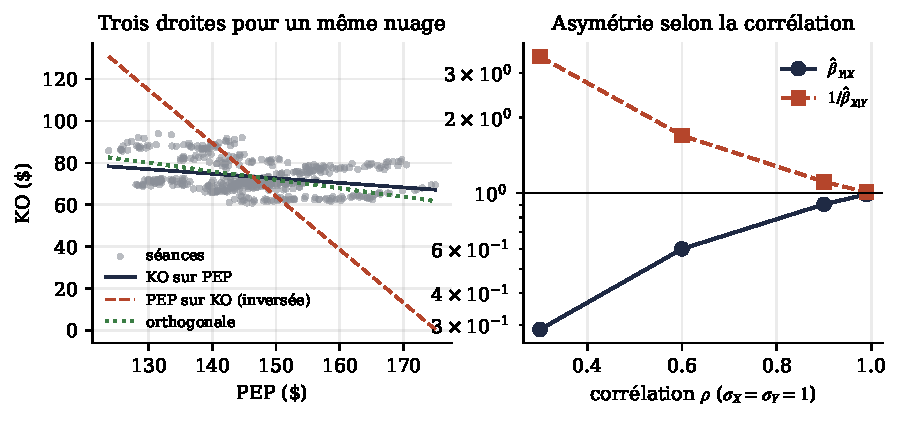
\includegraphics[width=0.95\textwidth]{ch02/asymetrie_regression.pdf}
\caption{À gauche, les cours de KO et PEP (500 séances) et trois droites d'ajustement : selon la méthode, le \og ratio de couverture\fg{} change du tout au tout, signe d'une relation inexistante. À droite, la pente directe et l'inverse de la pente réciproque ne coïncident que si la corrélation est proche de 1 (échelle logarithmique).}
\label{c2:fig:asym}
\end{figure}

\paragraph{Lecture pour le trading.} Quand la paire est réellement cointégrée (simulation), les trois estimateurs sont proches et convergent vers la vraie valeur ; quand elle ne l'est pas (KO/PEP sur cette période), ils divergent. \emph{L'écart entre $\hat\beta_{Y|X}$ et $1/\hat\beta_{X|Y}$ est donc un premier diagnostic gratuit} : s'il est grand, la relation est fragile. Les praticiens retiennent souvent la jambe la plus liquide comme $X$, ou testent les deux sens et gardent celui qui produit l'écart le plus stationnaire (chapitre~4).

\subsection{Prix ou log-prix ? Neutralité en parts ou en dollars}

Régresser les prix donne un ratio en \emph{nombre de parts} : $Y - \beta X$ est la valeur d'un portefeuille long une part de $Y$, court $\beta$ parts de $X$. Régresser les log-prix donne un ratio en \emph{élasticité} : $\log Y - \beta\log X$ ; une position \og neutre en dollars\fg{} (même montant investi des deux côtés) correspond à $\beta = 1$ en log. Le choix change la position et donc le risque : la version en log-prix est la plus courante en actions (on raisonne en rendements), la version en prix est naturelle pour deux instruments du même sous-jacent (or contre or), comme dans \texttt{atjte} où $k$ convertit des unités.

% =====================================================================
\section{Le maximum de vraisemblance}
% =====================================================================

\subsection{Principe}

Soit un modèle qui donne la densité des données $f(x_1,\dots,x_n;\theta)$ en fonction d'un paramètre $\theta$. La \emph{vraisemblance} est cette densité vue comme fonction de $\theta$, à données fixées : $\mathcal L(\theta) = f(x_1,\dots,x_n;\theta)$. L'estimateur du maximum de vraisemblance (MV) est la valeur de $\theta$ qui rend les données observées les plus probables. On maximise en pratique la log-vraisemblance $\ell(\theta) = \ln\mathcal L(\theta)$, plus simple (les produits deviennent des sommes) et qui a le même maximum car $\ln$ est croissante.

\begin{intuition}
Vous trouvez une pièce et la lancez dix fois : huit piles. Quelle probabilité de pile rend ce résultat le plus plausible ? Avec $p = 0{,}5$, huit piles est peu probable ; avec $p = 0{,}8$, c'est le résultat le plus probable. Le maximum de vraisemblance choisit $\hat p = 0{,}8$. C'est le même raisonnement, appliqué à un processus entier.
\end{intuition}

\subsection{Vraisemblance de l'AR(1)}

Pour l'AR(1) gaussien $X_t = c + \varphi X_{t-1} + \varepsilon_t$, $\varepsilon_t\iid\N(0,\sigma^2)$, la loi de $X_t$ \emph{sachant} $X_{t-1}$ est $\N(c+\varphi X_{t-1},\sigma^2)$. Par la formule des probabilités conditionnelles en chaîne, la densité jointe se factorise :
\[
f(x_0,\dots,x_n) = f(x_0)\prod_{t=1}^n f(x_t\mid x_{t-1}).
\]

\begin{proposition}\label{c2:prop:mlear1}
En ignorant le terme $f(x_0)$ (vraisemblance \og conditionnelle\fg), l'estimateur MV de $(c,\varphi)$ est l'estimateur MCO de $x_t$ sur $(1, x_{t-1})$, et $\hat\sigma^2_{MV} = \frac1n\sum_t \hat e_t^2$.
\end{proposition}
\begin{proof}
La log-vraisemblance conditionnelle vaut
\[
\ell(c,\varphi,\sigma^2) = \sum_{t=1}^n \ln\Big[\frac{1}{\sqrt{2\pi\sigma^2}}e^{-\frac{(x_t-c-\varphi x_{t-1})^2}{2\sigma^2}}\Big] = -\frac n2\ln(2\pi\sigma^2) - \frac{1}{2\sigma^2}\sum_{t=1}^n(x_t - c - \varphi x_{t-1})^2.
\]
Pour tout $\sigma^2$ fixé, maximiser en $(c,\varphi)$ revient à minimiser la somme des carrés : ce sont les MCO. On dérive ensuite par rapport à $\sigma^2$ : $-\frac{n}{2\sigma^2} + \frac{1}{2\sigma^4}\sum\hat e_t^2 = 0$, d'où $\hat\sigma^2 = \frac1n\sum\hat e_t^2$.
\end{proof}

La vraisemblance \emph{exacte} ajoute $\ln f(x_0)$, où $X_0 \sim \N\big(c/(1-\varphi),\,\sigma^2/(1-\varphi^2)\big)$ si le processus est stationnaire (proposition~\ref{c1:prop:ar1}). Ce terme pèse peu quand $n$ est grand, mais il pénalise les valeurs de $\varphi$ proches de 1 et améliore légèrement l'estimation sur échantillon court.

\paragraph{Propriétés asymptotiques.} Sous des conditions de régularité, l'estimateur MV est convergent et asymptotiquement normal, de variance égale à l'inverse de l'information de Fisher. Pour l'AR(1) stationnaire, cela donne $\Var(\hat\varphi) \approx (1-\varphi^2)/n$ \citep[ch.~5 et 8]{hamilton1994}.

\begin{codebox}[ — E3, MCO et maximum de vraisemblance]
\textbf{Protocole :} un AR(1) avec $c = 0{,}2$, $\varphi = 0{,}9$, $\sigma = 0{,}5$, $n = 300$ ; maximisation numérique (Nelder-Mead). \textbf{Résultats :} MCO : $\hat c = 0{,}1893$, $\hat\varphi = 0{,}9039$, $\hat\sigma = 0{,}5193$ ; MV conditionnel : exactement les mêmes valeurs ; MV exact : $\hat c = 0{,}1972$, $\hat\varphi = 0{,}9019$, $\hat\sigma = 0{,}5187$. La figure~\ref{c2:fig:ll} montre la log-vraisemblance profilée en $\varphi$.
\end{codebox}

\begin{figure}[h]
\centering
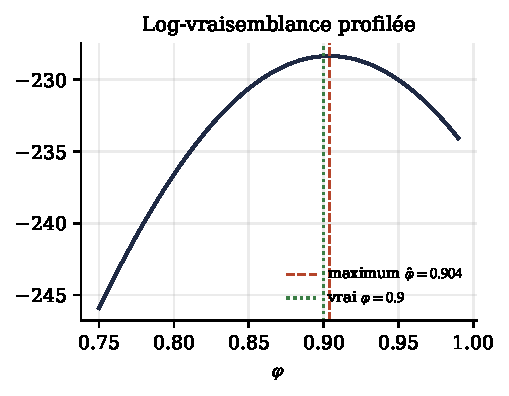
\includegraphics[width=0.48\textwidth]{ch02/vraisemblance_ar1.pdf}
\caption{Log-vraisemblance profilée de l'AR(1) en fonction de $\varphi$ (les autres paramètres sont optimisés pour chaque $\varphi$). Le maximum est proche, mais pas égal, à la vraie valeur : c'est l'incertitude d'estimation.}
\label{c2:fig:ll}
\end{figure}

% =====================================================================
\section{Le biais de petit échantillon et sa correction}
% =====================================================================

Le chapitre~1 (tableau~\ref{c1:tab:bias}) a mesuré que $\hat\varphi$ est biaisé vers le bas. L'approximation de \citet{kendall1954} donne $\E[\hat\varphi] - \varphi \approx -(1+3\varphi)/n$ quand la moyenne est estimée. On peut donc corriger :
\[
\hat\varphi_{c} = \hat\varphi + \frac{1+3\hat\varphi}{n}.
\]
La correction utilise $\hat\varphi$ au lieu de $\varphi$ (inconnu), ce qui laisse un petit biais résiduel.

\begin{codebox}[ — E4, correction de Kendall]
\textbf{Protocole :} $\varphi = 0{,}95$ (demi-vie vraie $13{,}51$), 3\,000 échantillons par taille. \textbf{Résultats} (tableau~\ref{c2:tab:kendall}) : la correction ramène la moyenne de $\hat\varphi$ très près de la vérité et supprime l'essentiel du biais de demi-vie, au prix d'une légère sur-correction de la médiane de la demi-vie quand $n$ est petit.
\end{codebox}

\begin{table}[h]
\centering\small
\caption{Estimation brute et corrigée de $\varphi = 0{,}95$ (moyennes et médianes sur 3\,000 échantillons).}
\label{c2:tab:kendall}
\begin{tabular}{rccccc}
\toprule
$n$ & $\overline{\hat\varphi}$ brut & $\overline{\hat\varphi_c}$ corrigé & demi-vie médiane brute & demi-vie médiane corrigée & écart-type de $\hat\varphi$\\
\midrule
100 & 0,9068 & 0,9430 & 7,92 & 14,61 & 0,0496\\
250 & 0,9336 & 0,9489 & 10,79 & 14,41 & 0,0247\\
1\,000 & 0,9462 & 0,9500 & 12,77 & 13,80 & 0,0105\\
\bottomrule
\end{tabular}
\end{table}

\begin{pitfall}
Corriger le biais ne réduit pas l'incertitude. Avec $n = 250$, l'écart-type de $\hat\varphi$ ($0{,}025$) reste du même ordre que la distance qui sépare $\varphi = 0{,}95$ de la racine unitaire $\varphi = 1$. Autrement dit, un an de données quotidiennes ne permet pas de distinguer de façon fiable un écart qui revient lentement d'un écart qui ne revient pas du tout. Le chapitre~3 quantifie ce problème de puissance.
\end{pitfall}

% =====================================================================
\section{Ce que la théorie apporte, et ses limites}
% =====================================================================

\paragraph{Apports.} Les MCO donnent le ratio de couverture à variance minimale et le \emph{spread} comme résidu ; le maximum de vraisemblance fournit un cadre unique pour estimer tous les modèles du cours (AR, Ornstein-Uhlenbeck, Kalman, copules) ; les erreurs-types robustes et la correction de biais rendent les estimations plus honnêtes.

\paragraph{Limites.} (1) Le ratio estimé dépend du sens de la régression, des unités et de la fenêtre ; il n'existe pas \og le\fg{} bon $\beta$. (2) Les hypothèses (H3)–(H4) sont presque toujours violées par les séries de prix. (3) Les propriétés asymptotiques du MV supposent que le modèle est juste ; si l'écart n'est pas un AR(1), l'estimateur converge vers le \og meilleur AR(1)\fg, pas vers une vérité. (4) Aucun estimateur ne crée de l'information absente des données : la précision est limitée par la longueur de l'échantillon, mesurée en nombre de demi-vies observées plutôt qu'en nombre de points.

% =====================================================================
\section{Fiche à recopier au tableau blanc}
% =====================================================================

\begin{whiteboard}
\begin{itemize}[leftmargin=1.2em]
\item \textbf{MCO simples :} $\hat b = \sum(x-\bar x)(y-\bar y)/\sum(x-\bar x)^2$, $\hat a = \bar y - \hat b\bar x$.
\item \textbf{MCO matriciels :} $\hat\beta = (X^\top X)^{-1}X^\top y$ ; $X^\top e = 0$ ; $\hat\sigma^2 = e^\top e/(n-k)$.
\item \textbf{Sans biais :} $\hat\beta = \beta + (X^\top X)^{-1}X^\top\varepsilon$ ; $\Var(\hat\beta) = \sigma^2(X^\top X)^{-1}$ sous (H4).
\item \textbf{Sandwich :} $(X^\top X)^{-1}\,\hat\Omega\,(X^\top X)^{-1}$ ; Newey-West : poids $1-j/(L+1)$.
\item \textbf{Asymétrie :} $\hat\beta_{Y|X}\hat\beta_{X|Y} = \hat\rho^2$.
\item \textbf{Orthogonale :} $s_{XY}b^2 + (s_{XX}-s_{YY})b - s_{XY} = 0$, racine de même signe que $s_{XY}$.
\item \textbf{Log-vraisemblance AR(1) :} $\ell = -\frac n2\ln(2\pi\sigma^2) - \frac1{2\sigma^2}\sum(x_t - c - \varphi x_{t-1})^2$ ; MV conditionnel $=$ MCO.
\item \textbf{Asymptotique :} $\Var(\hat\varphi)\approx(1-\varphi^2)/n$.
\item \textbf{Correction de Kendall :} $\hat\varphi_c = \hat\varphi + (1+3\hat\varphi)/n$.
\end{itemize}
\end{whiteboard}

% =====================================================================
\section{Exercices}
% =====================================================================

\begin{exercise}
Montrez que, dans la régression simple avec constante, la somme des résidus est nulle et que la droite passe par le point moyen $(\bar x,\bar y)$.
\end{exercise}

\begin{exercise}
Montrez que $R^2 = \hat\rho_{XY}^2$ en régression simple. Déduisez-en la proposition~\ref{c2:prop:asym} par un autre chemin.
\end{exercise}

\begin{exercise}
Vérifiez la proposition~\ref{c2:prop:tls} dans le cas $s_{XX} = s_{YY}$ : que vaut la pente orthogonale ? Interprétez géométriquement.
\end{exercise}

\begin{exercise}
Avec $\varphi = 0{,}95$ et $n = 250$, calculez l'écart-type asymptotique $\sqrt{(1-\varphi^2)/n}$ et comparez à l'écart-type mesuré dans le tableau~\ref{c2:tab:kendall}. Pourquoi l'asymptotique sous-estime-t-elle l'incertitude ?
\end{exercise}

\begin{exercise}[à coder]
Reprenez E2 en régressant $\log$KO sur $\log$PEP sur des fenêtres glissantes de 120 séances. Tracez le ratio dans le temps. Que conclure sur la stabilité de la \og couverture\fg{} ?
\end{exercise}

\begin{exercise}[à coder]
Implémentez un \emph{bootstrap} par blocs pour l'erreur-type de $\hat b$ dans E5 (tirage de blocs consécutifs de 25 observations) et comparez son taux de rejet à celui de Newey-West.
\end{exercise}

% =====================================================================
\section{Pour aller plus loin}
% =====================================================================

\begin{toread}
\begin{itemize}[leftmargin=1.2em]
\item \citet{hamilton1994}, chapitre~8 (\og Linear Regression Models\fg) pour les MCO et leurs propriétés ; chapitre~5 (\og Maximum Likelihood Estimation\fg) pour la vraisemblance des processus ARMA.
\item \citet{neweywest1987} : l'article original, très court, sur l'estimateur de variance robuste.
\item \citet{kendall1954} : la note originale sur le biais d'estimation de l'autocorrélation.
\item \citet{vidyamurthy2004} : la discussion du choix du ratio de couverture en \emph{pairs trading}, avant les tests de cointégration.
\end{itemize}
\end{toread}

\section{Scripts du chapitre}
\noindent\texttt{code/ch02/ch02\_regression.py} : E1 (MCO à la main contre \texttt{statsmodels}), E2 (asymétrie et figure~\ref{c2:fig:asym}), E3 (vraisemblance et figure~\ref{c2:fig:ll}), E4 (tableau~\ref{c2:tab:kendall}), E5 (Newey-West). Résultats : \texttt{code/ch02/results.json}.
